\documentclass[11pt]{article}
\usepackage[a4paper,margin=24mm]{geometry}
\usepackage{fontspec}
\setmainfont{Noto Serif}
\usepackage{microtype}
\usepackage{amsmath,amssymb}
\usepackage{booktabs}
\usepackage{longtable}
\usepackage{graphicx}
\usepackage{xurl}
\usepackage{hyperref}
\usepackage{bookmark}
\hypersetup{colorlinks=true,linkcolor=blue,citecolor=blue,urlcolor=blue}
\urlstyle{same}
\setlength{\parindent}{0pt}
\setlength{\parskip}{5pt}
\setlength{\emergencystretch}{3em}
\newcommand{\doctype}{Working manuscript}
\newcommand{\docversion}{v0.04}
\newcommand{\docdate}{12 November 2026}
\newcommand{\versiondoi}{not-assigned}
\newcommand{\conceptdoi}{not-assigned}
\newcommand{\docrepo}{github.com/fsantibanezleal/CAOS\_Geophysics}
\newcounter{algorithm}
\newenvironment{algorithm}[1]{%
  \refstepcounter{algorithm}%
  \begin{center}\begin{minipage}{0.96\textwidth}\hrule\vspace{5pt}%
  \textbf{Algorithm \thealgorithm. #1}\par\vspace{4pt}\hrule\vspace{4pt}%
}{\vspace{4pt}\hrule\end{minipage}\end{center}}
\newcommand{\headerblock}{%
\begin{center}
\fbox{\parbox{0.94\textwidth}{\small\raggedright
\textbf{\doctype} \quad$\cdot$\quad \docversion, \docdate \quad$\cdot$\quad Licence CC BY 4.0\\[2pt]
CAOS Research open-problems programme \quad$\cdot$\quad product Inverse Earth Studio \quad$\cdot$\quad first-arrival tomography\\[2pt]
Version DOI: not assigned\\[2pt]
Concept DOI: not assigned\\[2pt]
Not peer reviewed. Source code, data and computational records: \href{https://github.com/fsantibanezleal/CAOS_Geophysics}{\texttt{\docrepo}}
}}
\end{center}
\vspace{4pt}}
\title{Geometry-normalized learned first-arrival tomography and null-space correction: two synthetic studies}
\author{Felipe Santib\'a\~nez-Leal}
\date{}
\begin{document}
\maketitle
\headerblock

\begin{abstract}
Learned inverse maps can return velocity perturbations that fit their training distribution but disagree with an acquisition operator. The frozen supervised residual correction failed its joint family-and-acquisition comparison: learned-to-L2 velocity RMSE was 1.0437 and independent travel-time RMSE was 1.3961. A separate synthetic follow-up projects that frozen estimate's slowness correction into the null space of a straight-ray path-length matrix and applies bounded velocity conversion. The projected candidate beats the L2 baseline in both aggregate metrics in all four fixed cohorts, but a same-case raw-versus-projected analysis exposes a trade-off: on joint shift, projected/raw error ratios are 0.9177 for velocity (paired 95\% interval 0.9123--0.9230) and 0.7080 for independent travel time (0.6954--0.7213); on ID cases, the velocity ratio is 1.9583 while the travel-time ratio is 0.9290. Projection therefore changes the balance of model and data error rather than uniformly improving the raw CNN. A calibration-only threshold reanalysis uses 1.0649 ms and flags 160 of 160 joint-shift cases; this is not field accuracy. Current-source CUDA training and CPU replay verify the frozen synthetic protocols. The evidence does not establish a new null-space algorithm, field transfer, geological recovery or superiority to published tomography methods.
\end{abstract}

\section{Introduction}
First-arrival tomography estimates a spatial velocity field from source--receiver travel times. Finite acquisition geometry leaves model directions weakly constrained or unobservable. An inverse solution therefore depends on its parameterization, regularization, starting model and data coverage, rather than on travel times alone. A visually coherent model does not establish that the data identify its internal structure.

Regularized tomography addresses this ill-posedness through an explicit forward operator. Learned methods add data-distribution priors, parameterize the inverse map, or impose wave-propagation physics during optimization. Examples include supervised networks motivated by the structure of circular tomography \cite{fan_ying_2023}, physics-informed eikonal inversion \cite{waheed_2021}, neural-network parameterization with ensemble Kalman inversion \cite{eki_nn_2024}, and recent multiparameter and residual PINN formulations \cite{song_2025,msp_respinns_2026}. These approaches differ in their inputs, governing equations and optimization; they are not interchangeable baselines.

The inverse-problem language matters here because several different questions are often collapsed into one map image. A model can have low velocity RMSE against a synthetic truth and still predict travel times that disagree with the observed data. Conversely, a model may fit the data while being far from the generator truth along directions the survey does not resolve. Classical resolution analysis distinguishes data fit, parameter resolution and model uncertainty; these are related but not interchangeable quantities \cite{backus_gilbert_1968,menke_2012,aster_2018}. First-arrival travel time itself is also an approximation to wave propagation. Ray theory treats travel time as an integral along a path; finite-frequency sensitivity occupies a region around the geometrical ray, and wavefront solvers account for first arrivals through eikonal approximations \cite{vidale_1988,hole_1992,podvin_lecomte_1991,dahlen_2000,dahlen_resolution_2004}. The experiments described below use straight rays for the inverse and a second fixed-ray discretization for scoring. They do not evaluate finite-frequency effects or refracted paths.

The earlier experiment was designed as a supervised residual correction around a matched regularized straight-ray inverse. Its locked result is not a clean claim that all learned residuals fail: the velocity map is better than the regularized L2 map on ID and acquisition-layout cases, while its independently evaluated travel-time errors are worse in every recorded cohort. The family and joint shifts also worsen velocity error. This distinction is the main scientific reason to report both domains, to retain every cohort, and to avoid describing a visually sharper learned image as a physical improvement. A learned map induces a distribution-dependent regularizer through its weights and training set, but the training distribution does not supply new measurements in the nullspace of an unseen acquisition.

Null-space projection is also established. Pratt used null-space model components to incorporate a priori information into cross-hole travel-time inversion \cite{pratt_1997}; later work used null-space projection to explore non-uniqueness in magnetotellurics \cite{chave_2007}. The present computation therefore does not claim to introduce null-space projection. It asks a narrower empirical question: when a frozen learned estimate is available, does projecting its slowness correction against the acquisition's straight-ray operator improve two matched aggregate criteria relative to a straight-ray L2 solution on fixed synthetic cohorts?

Recent learned-inverse work makes the novelty boundary still narrower. Jacome et al. introduce nonlinear, sensing-specific null-space projections learned with neural networks and study them across several computational-imaging problems, including theoretical guarantees \cite{jacome_npn_2025}. Bacca's 2025 preprint studies a different projection correction that enforces measurement consistency for learned reconstructions and analyzes when that correction becomes the identity \cite{bacca_projection_2025}. These are related ideas, not methods reproduced or benchmarked here. The present experiment takes one frozen learned velocity estimate, converts its correction to slowness, applies an SVD-defined linear orthogonal projection for a fixed straight-ray matrix, and converts back with bounds. It does not learn a nonlinear null-space prior, establish a convergence or reconstruction theorem, or compare against either published method. Because clipping and nonlinear conversion follow the linear projection, the projected term's annihilation under the path matrix is not a guarantee of the final nonlinear model's data consistency.

That question is deliberately narrower than a comparison of current tomography systems. The supervised map, a PINN that minimizes the eikonal residual, an ensemble inversion, a fast-marching objective and a full-waveform method have different forward physics, data access and uncertainty semantics. They cannot be ranked by placing unrelated published metrics in one table. The analysis therefore reports the product's paired comparison and uses the literature to define method boundaries, not to imply a benchmark against current published systems. A fair head-to-head study would require common shot geometry, noise realization, parameterization, training information, parameter-selection budget, forward solvers and scoring, plus independent reproductions. None is available in this data package.

The research contribution is an evaluation of a proposed hybrid and its evidence boundary, not a new inverse theory. The original follow-up compared only the projected candidate with L2, which hid the incremental effect of the projection. A post-hoc reconstruction now evaluates raw and projected predictions on identical held-out cases, with alpha fixed by the original calibration receipt. This conditional intervention shows the projection's effect within the declared synthetic simulator: it lowers the independent travel-time error in every cohort, while its effect on velocity error changes sign between the in-distribution/acquisition-shift cohorts and the family/joint-shift cohorts. Paired case intervals quantify variability within those fixed sets only. These data support a more discriminating ablation; they do not turn the synthetic effect into a population-level or field claim.

\section{Related work and comparison scope}\label{sec:related-work}
First-arrival tomography has a long-established family of ray-based formulations. Aki and Lee's local-earthquake inversion illustrates how travel-time observations constrain spatial velocity anomalies through a sensitivity operator; later reviews describe the interaction among ray coverage, parameterization, regularization and nonlinear path updates across crustal and lithospheric applications \cite{aki_lee_1976,rawlinson_sambridge_2003}. Controlled-source studies have compared inversion strategies on real acquisition geometries and have treated resolution as a spatially varying property rather than a global image-quality score \cite{zelt_barton_1998,zelt_resolution_1998}. These studies motivate the present paper's matched geometry, explicit baseline, and separation of model-space truth error from travel-time prediction error. They do not provide numerical targets that can be transferred to our 16-by-16 synthetic grid.

The baseline here is a quadratic straight-ray inverse in slowness. It is intentionally transparent and computationally stable, but it is not a substitute for a modern nonlinear first-arrival workflow that updates rays, solves an eikonal equation, estimates source terms, or uses a survey-specific mesh. Fast marching and finite-difference eikonal solvers answer a different forward question from a fixed path-length matrix \cite{vidale_1988,podvin_lecomte_1991}. PINNeik addresses neural solution of the eikonal forward problem, while PINNtomo and later physics-informed tomography studies optimize velocity and travel-time fields under their own physical losses \cite{pinneik_2021,waheed_2021,song_2025}. A comparison to those approaches would require the same data, geometry, parameterization, tuning budget and held-out scoring; no such comparison is performed here.

Learned inverse maps and neural parameterizations offer alternative ways to encode priors. Published travel-time learning, ensemble Kalman inversion, and sparse-ray neural inversion differ in training supervision, forward model and uncertainty treatment \cite{fan_ying_2023,eki_nn_2024,volcano_ann_2024}. OpenFWI provides a large multi-structure benchmark for full-waveform inversion, which is valuable for that problem but is not a first-arrival travel-time benchmark and cannot serve as a direct comparator for this experiment \cite{openfwi_2022}. The distinction matters: similarity of the target quantity (velocity) does not make different wave physics, acquisition, or losses interchangeable.

Null-space reasoning is also established in geophysical inverse theory. Perturbations in weakly observed model directions can be large while producing little change in the modeled data, and null-space exploration has been used to characterize nonuniqueness in both seismic and magnetotelluric settings \cite{backus_gilbert_1968,pratt_1997,chave_2007}. More recent learned null-space and data-proximal frameworks formalize how a learned correction can be restricted by an operator or a prescribed data-error tolerance \cite{jacome_npn_2025,goeppel_2023}. The present implementation is narrower: it projects a frozen CNN's correction using the right singular vectors of one discretized straight-ray matrix, then converts the result from slowness to bounded velocity and scores it with a separate bilinear operator. Because the velocity map is nonlinear, this construction is not an exact data-consistency guarantee for the final velocity model. It is an algorithmic intervention evaluated empirically, not a new theorem or a reproduction of the cited networks.

This comparison therefore addresses a specific gap in the product's evidence record: whether the already-selected projection changes same-case CNN errors, in addition to whether the projected model beats the L2 reference. The two questions need separate denominators. Projected-to-L2 ratios assess the candidate against the classical baseline; projected-to-raw ratios isolate the incremental computation conditional on one checkpoint, calibration and generator. Neither ratio establishes the quality of the model as an image, and neither is a field performance estimate.

\section{Projection theory and operator distinctions}\label{sec:theory}
Let the linearized discretized observation map be $A\in\mathbb{R}^{m\times n}$ and let $s\in\mathbb{R}^n$ be cell slowness. In the experiment, each entry of $A$ is a straight-ray path length through one cell, so $As$ has travel-time units. With noisy observations $y$, a classical reference estimate minimizes a weighted data residual and a quadratic smoothness penalty around a reference model:
\begin{equation}\label{eq:l2-objective}
\hat{s}_{\lambda}=\arg\min_s\;\|W^{1/2}(As-y)\|_2^2+\lambda\|L(s-s_0)\|_2^2.
\end{equation}
Here $W$ is the observation weighting, $L$ is the declared regularization operator, and $\lambda$ is selected using calibration cases only. This convex objective defines the baseline for a fixed $A$, $W$, $L$ and $\lambda$; it does not imply that the recovered parameter vector is unique when the augmented normal operator is rank deficient.

For a singular-value decomposition $A=U\Sigma V^{\mathsf T}$, retain the right singular vectors associated with the study's declared numerical rank. If $V_r$ contains those vectors and $V_0$ spans the retained numerical null space, the orthogonal projector used for a correction is
\begin{equation}\label{eq:nullspace-projector}
P_0=V_0V_0^{\mathsf T}=I-V_rV_r^{\mathsf T},\qquad P_0^{\mathsf T}=P_0,\qquad P_0^2=P_0.
\end{equation}
For a perturbation $\delta s$, $P_0\delta s$ is orthogonal to the retained row-space basis. In exact arithmetic under the same rank convention, $AP_0\delta s=0$. With finite precision and a truncated SVD, the actual numerical claim is bounded by the measured residual $\|AP_0\delta s\|$ and the recorded singular-value cutoff. The rank, nullity and residual diagnostics in the results are thus checks on the implemented matrix and tolerance. They are not a physical resolution analysis of the subsurface.

The algorithm first computes a calibrated classical estimate $\hat{s}_{\lambda}$ and a frozen CNN prediction $s_{\mathrm{cnn}}$. It forms a learned correction relative to the baseline and scales its projected component by the calibration-selected $\alpha$:
\begin{equation}\label{eq:projected-slowness}
s_{\mathrm{proj}}=\hat{s}_{\lambda}+\alpha P_0(s_{\mathrm{cnn}}-\hat{s}_{\lambda}).
\end{equation}
The retained setting is $\alpha=1.0$. This expression makes the intervention explicit: the raw CNN output is not added wholesale, and the projection does not retrain or alter the network. It also clarifies why the calibration sweep is not itself a comparison to an unprojected network. A calibration-selected $\alpha$ controls the magnitude of the projected residual; only same-case predictions with and without $P_0$ identify the corresponding computational contrast for a fixed checkpoint.

Physical display and scoring use velocity, not an unconstrained slowness vector. The slowness field is converted cellwise and bounded according to the frozen physical interval:
\begin{equation}\label{eq:slowness-velocity}
v_j=\operatorname{clip}\!\left(\frac{1}{s_j},v_{\min},v_{\max}\right),\qquad j=1,\ldots,n.
\end{equation}
Reciprocal conversion and clipping are nonlinear. Therefore $A(s_{\mathrm{proj}}-\hat{s}_{\lambda})\approx0$ does not entail that the converted velocity has unchanged travel times, especially where the perturbation is large or clipping is active. No clipping occurred in the recorded null-space runs, but the reciprocal map alone remains nonlinear. The independent bilinear travel-time oracle is retained precisely to evaluate this post-projection model without assuming that nullity of $A$ guarantees data-space invariance.

The study reports model-space velocity RMSE against synthetic truth and data-space error through the independent oracle. For case $k$, these are $e_{v,k}=\sqrt{n^{-1}\sum_j(v_{k,j}-v^*_{k,j})^2}$ and $e_{t,k}=\sqrt{q^{-1}\sum_i(\mathcal{F}_{Q}(v_k)_i-y_{k,i})^2}$, where $\mathcal{F}_{Q}$ is the separately discretized bilinear forward calculation. A ratio of cohort means is reported as
\begin{equation}\label{eq:ratio-of-means}
R_e=\frac{N^{-1}\sum_{k=1}^{N}e_{e,k}^{(\mathrm{candidate})}}{N^{-1}\sum_{k=1}^{N}e_{e,k}^{(\mathrm{reference})}},\qquad e\in\{v,t\}.
\end{equation}
Thus $R_e<1$ is favorable only for the named metric and denominator. A paired case bootstrap resamples the same case identifiers in numerator and denominator within each fixed cohort. Its interval describes resampling variation over that cohort's cases; it does not include uncertainty over training seeds, alternative generators, geological populations, acquisition redesign or field error. The analysis code preserves the distinction between these conditional intervals and uncertainty in a target population.

The numerical projector depends on a finite-dimensional $A$, a rank threshold and a chosen cell basis. Changing discretization, ray tracing, path bending, weighting, topography or mesh changes the row space and therefore changes $P_0$. A null direction under one fixed straight-ray matrix need not be a null direction for a nonlinear eikonal operator or a finite-frequency wave operator. We consequently use the phrase “null space of the discretized straight-ray matrix” throughout. We do not infer that the model perturbation is invisible to all physical observations or that every cell outside the row space is unconstrained in a realistic survey.

For the independent nonlinear travel-time oracle $\mathcal{F}_{Q}$, a small velocity perturbation $\delta v$ changes the predicted data to first order according to its local Jacobian $J_Q(v)$:
\begin{equation}\label{eq:oracle-linearization}
\mathcal{F}_{Q}(v+\delta v)-\mathcal{F}_{Q}(v)=J_Q(v)\,\delta v+\mathcal{O}(\|\delta v\|_2^2).
\end{equation}
The projector is constructed from $A$ in slowness coordinates, whereas the diagnostic above concerns a different operator acting on velocity perturbations. Neither the Jacobian nor its null space is constrained to coincide with $A P_0$. This operator distinction is the reason a low matrix residual is necessary for verifying the projection implementation but insufficient for claiming data consistency of the final prediction.

For each geometry, the numerical projector check records the largest residual over the generated projected corrections. If $\tau_A$ is the declared residual tolerance and $\epsilon_{\mathrm{svd}}$ the SVD rank threshold, the implementation check is of the form
\begin{equation}\label{eq:projection-check}
\max_k\|A P_0\delta s_k\|_{\infty}\leq\tau_A,
\qquad \sigma_i>\epsilon_{\mathrm{svd}}\sigma_1\;\;\text{for retained singular modes}.
\end{equation}
This is a finite numerical contract. It does not quantify the spatial resolution kernel, because the experiment does not invert a realistic survey using a ray-updating tomography engine, and its synthetic target is known by construction.

The paired bootstrap interval for a cohort is obtained by sampling $N$ case indices with replacement on each draw $b$ and recomputing the ratio from the paired errors. Writing $I_b$ for the sampled indices, the statistic is
\begin{equation}\label{eq:paired-bootstrap}
R_e^{(b)}=\frac{\sum_{k\in I_b} e_{e,k}^{(\mathrm{proj})}/N}{\sum_{k\in I_b}e_{e,k}^{(\mathrm{raw})}/N},\qquad b=1,\ldots,B.
\end{equation}
The reported endpoints are the empirical 2.5th and 97.5th percentiles over $B=20{,}000$ deterministic PCG64 draws. This resampling keeps numerator and denominator paired by case. It is narrower than a hierarchical design that would resample training runs and generator families, which are not replicated here; it must not be interpreted as a confidence interval for future field surveys.

\section{Inverse problem and correction}\label{sec:inverse-problem-and-correction}
The earlier model is a residual CNN conditioned on a deterministic straight-ray inverse and two measured-geometry channels. Let $v_{\mathrm{ref}}$ be the fixed reference velocity, $t_i$ an observed travel time and $\ell_i=\sum_j A_{ij}$ the length of ray $i$. The ray residual feature is $q_i=(t_i-(A v_{\mathrm{ref}}^{-1})_i)/\ell_i$, which has slowness units. For cell $j$ with coverage $c_j=\sum_i A_{ij}>0$, the corrected backprojection feature is
\[
  b_j=-\frac{v_{\mathrm{ref},j}^2}{400\;\mathrm{m/s}}\frac{\sum_i A_{ij}q_i}{c_j},
  \qquad z_j=\frac{c_j}{\max_k c_k}.
\]
The feature builder also supplies the deterministic inverse $v_0$ as the first channel, normalized as $(v_0-v_{\mathrm{ref}})/(400\;\mathrm{m/s})$. The three-channel network predicts a residual $\Delta v=250\tanh f_\theta((v_0-v_{\mathrm{ref}})/400,b,z)$ and returns $\hat v=\Pi_{[1400,4000]}(v_0+\Delta v)$. Its final convolution is zero-initialized, so the initial prediction is the deterministic inverse, subject to the same physical bounds. This corrected feature addresses a dimensional defect in an earlier residual input, but the frozen joint-shift test still performs worse than the matched straight-ray L2 baseline (Section~4). This paper evaluates a later null-space correction using the frozen learned estimate; it proposes no new null-space method.

\subsection{Feature derivation, units, and inference boundary}
The three input channels have different roles and different physical interpretations. The first channel, $v_0$, is a reproducible classical reconstruction for the same source--receiver geometry. It provides a stable starting field and avoids asking the network to infer the entire background velocity from a sparse list of picks. The second channel, $b$, is a geometry-weighted correction proxy computed from the residual between observed arrivals and the reference prediction. The third channel, $z$, encodes ray coverage, normalized by its maximum over the grid. Coverage communicates where the acquisition has accumulated path length; it is not a posterior variance or a direct measure of resolution.

The dimensional normalization is designed so the network does not receive a raw time residual whose scale changes with the length of each path. Dividing by $\ell_i$ maps the residual to a travel-time-per-distance quantity, consistent with slowness. Accumulating these values through $A_{ij}$ and dividing by $c_j$ forms a path-weighted local average. Multiplication by $v_{\mathrm{ref},j}^2$ converts a slowness perturbation to a first-order velocity perturbation because $\mathrm{d}(1/v)/\mathrm{d}v=-1/v^2$; division by the fixed 400 m/s scale makes the channel numerically comparable to the normalized deterministic inverse. The leading minus sign follows the same derivative. The actual CNN remains nonlinear and is trained against velocity targets, so this feature is an input representation rather than a closed-form update.

For a ray with observed time $t_i$ and reference model $s_{\mathrm{ref}}$, the scalar residual channel is
\begin{equation}\label{eq:normalized-ray-residual}
q_i=\frac{t_i-\sum_j A_{ij}s_{\mathrm{ref},j}}{\ell_i},\qquad [q_i]=\mathrm{s/m}.
\end{equation}
For cell $j$, the coverage-weighted feature is then
\begin{equation}\label{eq:coverage-backprojection}
b_j=-\frac{v_{\mathrm{ref},j}^{2}}{400\;\mathrm{m/s}}\frac{\sum_i A_{ij}q_i}{c_j},\qquad z_j=\frac{c_j}{\max_k c_k}.
\end{equation}
The units of $b_j$ are dimensionless after the declared normalization: $A_{ij}q_i/c_j$ has units s/m, while $v^2/(400\;\mathrm{m/s})$ has units m/s. Cells with zero coverage require an explicit finite-value policy in the feature builder; they cannot be assigned an unobserved correction by dividing by zero. The implementation uses the validated coverage handling in the source module and retains the geometry channel so an unilluminated cell is not silently treated as equivalent to a well-sampled cell.

The normalized velocity residual added to the baseline is
\begin{equation}\label{eq:bounded-cnn-update}
\Delta v=250\;\mathrm{m/s}\;\tanh f_{\theta}(x_0,b,z),\qquad \hat v=\Pi_{[1400,4000]\,\mathrm{m/s}}(v_0+\Delta v),
\end{equation}
where $x_0=(v_0-v_{\mathrm{ref}})/(400\;\mathrm{m/s})$ and $f_\theta$ is the three-channel convolutional map. The hyperbolic tangent bounds the learned residual before it is added to the baseline; the final projection imposes the experiment's velocity interval. The last convolution is initialized to zero, so an untrained network starts at the deterministic estimate instead of an arbitrary field. This initialization stabilizes the starting point, but does not guarantee that training improves generalization or that each output cell is resolved.

The distinction between input scale, output scale and physical bound is material. The 400 m/s feature scale normalizes the baseline and maps a first-order slowness correction; the 250 m/s factor limits the learned residual before physical clipping; and the 1400--4000 m/s interval is the generator's declared model domain. None of these constants is estimated from a field survey. Rescaling them changes the function class and optimizer conditioning. A valid replication must preserve these values or treat each change as a separate experimental method with a new frozen evaluation.

The CNN receives the geometry-normalized channels and is trained on paired synthetic velocity models and generated travel-time observations. The case split, training seed, optimizer, epoch ceiling, patience rule, gradient cap and validation checkpoint are specified in the frozen protocol below; the test cohorts are not used for these choices. The network's loss is a model-space supervised objective, whereas the paper also evaluates its output with a separate forward-time score. This difference is intentional: optimizing model RMSE does not automatically optimize forward prediction, and checking only the supervised loss would conceal the central failure of this checkpoint under joint shift.

This feature formulation is the product's proposed method hypothesis: physically scaled residual information plus a coverage channel might help a bounded learned correction across acquisition and family shifts. The locked study does not support that hoped-for advantage. The CNN improves neither the joint-shift velocity criterion nor the independent travel-time criterion relative to the matched straight-ray baseline, and the per-case threshold flags every joint-shift case. Consequently, this section documents the proposed method and its falsification conditions; it is not evidence that the feature engineering succeeded or that the architecture represents the current state of the art.

The hypothesis is falsifiable because it requires simultaneous improvement in model and data space on a cohort whose geology family and acquisition differ from training. A lower training loss, an attractive velocity section, or reduced error on familiar geometries would not satisfy that requirement. The threshold screen is reported separately from the ratio rule: it asks whether a held-out prediction exceeds the calibration-derived tolerance, while the paired ratios compare two methods on the same fixed cases. These checks answer different questions and are not combined into an unregistered pass score. The frozen joint-shift result fails both criteria, so subsequent figures retain the failed outcome rather than selecting a more favorable cohort or redefining the threshold.

The feature channels also do not make acquisition bias disappear. The normalized backprojection averages measured residuals over cells reached by the straight rays, but the residual itself contains observation noise, operator mismatch and any inadequacy of the reference model. A coverage channel tells the network where path length accumulates; it does not tell the network which ray is trustworthy or how uncertainty varies by pick. The training examples can therefore teach correlations between coverage and the authored model families without learning a transferable physical law. The paper's split design tests specific held-out family and layout changes, but it does not isolate noise, geometry, prior bias or target-family complexity as causal factors.

Likewise, a residual CNN that starts at the deterministic inverse is not guaranteed to preserve the classical objective. Its learned update is bounded in velocity space, while the L2 estimator is obtained in slowness space and the scorer acts through a separate bilinear operator. Those spaces and operations are not equivalent under reciprocal conversion. The matched baseline remains the appropriate comparator for the stated product hypothesis, but disagreement between the network and that baseline cannot by itself identify which estimate is closer to a field model. Synthetic truth supplies one controlled answer for the authored cases; field calibration, independent surveys and a broader family of inverses are needed for a practical conclusion.

The later null-space operation acts on this already frozen CNN output. It does not reuse the learned feature map to compute a new inverse, modify the checkpoint, or supply new geological information. The distinction lets the paper attribute claims correctly: the M12 learned inverse fails its predeclared comparison, whereas the separate v1.1 study asks whether a projected variant of that frozen estimate can improve on a selected classical reference within another fixed synthetic design. The paired ablation is confined to this latter design and cannot rescue or overturn the earlier M12 test.

\subsection{Relation between the two frozen experiments}
The residual-v3.1 model and null-space v1.1 follow-up use the same checkpoint identity but different seed namespaces and different calibration structure. The primary learned study assesses a geometry-normalized CNN against L2 on its original held-out splits. The null-space study calibrates $\lambda$ and $\alpha$ using its own disjoint calibration cases, then scores four new cohorts. That separation avoids representing the follow-up as a reanalysis of the original test set, but it also means the two receipts cannot be combined into one pooled estimate. We report their outcomes in separate tables and state explicitly which one is the locked failure and which one is an exploratory correction study.

The same checkpoint does not make the experiments statistically paired. A paired contrast requires the same synthetic case, observation noise, target model and score function in both conditions. This is why the new projection counterfactual regenerates raw and projected outputs inside the v1.1 test cohorts, rather than subtracting scores from the earlier v3.1 receipt. The independent case IDs and seed manifests provide the required matching for this narrow intervention. They do not create paired evidence between the two studies, and the independent-oracle metric should not be confused with the straight-ray objective used to choose the L2 reference.

For a fixed acquisition, let $A\in\mathbb{R}^{n_d\times n_m}$ contain cell lengths traversed by each straight source--receiver ray. For slowness $s=1/v$, the linearized travel-time model is $t=As$. A regularized straight-ray estimate $s_c$ is compared with a learned velocity estimate $v_\ell$ from a frozen CNN checkpoint. The learned correction in slowness is
\[
  \delta s_\ell = v_\ell^{-1}-s_c.
\]
Let $N$ have orthonormal columns spanning $\ker(A)$, obtained from a full singular-value decomposition with a machine-precision rank tolerance. The orthogonal projector $P_N=NN^\mathsf{T}$ gives the candidate
\[
  s_\alpha = \operatorname{clip}\!\left(s_c+\alpha P_N\delta s_\ell,
                 1/4000,1/1400\right), \qquad v_\alpha=s_\alpha^{-1}.
\]
The projection satisfies $A P_N\delta s_\ell\simeq 0$ before clipping, to numerical precision. Clipping and reciprocal conversion are nonlinear; consequently the final candidate need not preserve travel times exactly. The code checks the basis residual and records the projected-correction residual and clipped fraction for each acquisition.

For calibration, $\alpha$ is selected from $\{0,0.25,\ldots,2\}$. A candidate is eligible only if both its velocity RMSE and its independent forward travel-time RMSE are below the straight-ray L2 result. Among eligible values, the smallest mean of those two ratios is selected, with the smaller $\alpha$ resolving ties. If none qualifies, $\alpha=0$ returns the straight-ray L2 baseline. Test-cohort scores do not select $\alpha$.

The recorded calibration curve makes the trade-off and selection criterion inspectable (Figure~\ref{fig:calibration}). Velocity error reaches its minimum at the selected $\alpha=1.0$ and rises at larger corrections, whereas travel-time error decreases gradually over the tested grid. The selection is therefore not equivalent to minimizing velocity error alone: both criteria and a strict improvement over baseline determine eligibility, and no held-out cohort contributes to this choice.

This post-hoc rule is distinct from training a neural network with an eikonal residual, learning a travel-time-to-slowness inverse map, or estimating an ensemble posterior. It also differs from the established use of null-space components to inject external prior structure: here the candidate direction is supplied by a learned estimate. No theorem states that its projection improves nonlinear travel times or velocity error.

\section{Synthetic protocol}
The source checkpoint is the earlier residual-correction model. The frozen protocol used 1,200 training cases (seeds 217001--218200), 160 validation cases (227001--227160), 160 ID cases (237001--237160), 80 family-only cases (247001--247080), 80 acquisition-only cases (257001--257080), and 160 joint-OOD cases (267001--267160). Training families were layered, lens and dipping with layouts A/B; the family holdout used fault/salt on A/B, the acquisition holdout used training families on layout C, and the joint holdout used fault/salt on C. Adam used seed 77214, learning rate $5\times10^{-4}$, batch size 64, maximum 100 epochs, patience 20 and gradient-norm cap 5. Validation selected epoch 100 and L2 regularization $\lambda=100$. The locked table reports the archived ratios, not a replay performed for the current study. The joint-OOD ratios were 1.0437 for velocity RMSE and 1.3961 for independent travel-time RMSE; thus the checkpoint fails the requirement that both ratios be below one.

The null-space follow-up uses that frozen checkpoint and an independently frozen calibration cohort of 160 realizations plus four new test cohorts: 160 in-distribution, 80 family-only shift, 80 acquisition-only shift and 160 joint family-and-acquisition shift. Their seed bases are 417001, 427001, 437001, 447001 and 457001. These seed namespaces are disjoint from the earlier M12 studies. The training and null-space studies therefore do not form a paired comparison with each other. Within the null-space follow-up itself, however, the exact checkpoint and seed manifests permit regeneration of raw CNN predictions for the same four test cohorts. The post-hoc analysis in Section~\ref{sec:paired-ablation} applies the calibration-selected alpha without retuning and compares raw and projected outputs against identical truth and observations. It does not modify the original v1.1 receipt or its projected-to-L2 verdict. The 6 November 2026 source-current reproduction retains the checkpoint and receipts; the 12 November verifier run reproduced five residual and four null-space cohorts. The separate counterfactual receipt binds the generated same-case scores and bootstrap intervals to the source hashes.

Velocity RMSE is computed against the synthetic generator's true velocity. Travel-time error is computed with an independent bilinear forward operator rather than reusing only the straight-ray matrix used for projection. Ratios are projected-candidate RMSE divided by straight-ray L2 baseline RMSE; values below one favor the projected candidate for that aggregate metric. The 95\% intervals resample paired case identifiers with replacement and calculate the ratio of mean per-case RMSEs on each of 20,000 draws using NumPy PCG64, seed 6122026 and linear quantiles. They quantify resampling variation within each fixed generator cohort, not variation across geological settings.

The archived scorer passed an infinite value as its forward-threshold parameter, so its stored zero-exceedance fields are invalid threshold results. A separate post hoc calculation applies one threshold, 1.0649004873 ms, defined as the 95th percentile of calibration learned-oracle RMSE and held fixed across all cohorts. Table~\ref{tab:threshold-reconciliation} reports the resulting counts from the retained per-case errors. It flags 160 of 160 joint-shift cases and 80 of 80 family-shift cases, while only 3 of 80 acquisition-shift cases exceed the threshold. These are synthetic cohort diagnostics derived from an oracle error, not a field detector, calibrated probability or measure of geological accuracy; they do not change the RMSE comparison or the study's evidence limits.

\begin{table}[htbp]
\centering
\caption{Calibration-derived threshold flags computed from retained synthetic learned-oracle errors; they are diagnostic counts, not field accuracy.}
\label{tab:threshold-reconciliation}
\begin{tabular}{lrrr}
\toprule
Cohort & $n$ & Exceedances & Rate \\
\midrule
Calibration & 160 & 8 & 5.000\% \\
In-distribution test & 160 & 7 & 4.375\% \\
Family-shift test & 80 & 80 & 100.000\% \\
Acquisition-shift test & 80 & 3 & 3.750\% \\
Joint-shift test & 160 & 160 & 100.000\% \\
\bottomrule
\end{tabular}
\end{table}


The historical compatibility replay verified the hash-bound metric computation over four cohorts, but its original external run directory was later superseded by the current-source reproduction. On 6 November 2026, the frozen residual-v3.1 checkpoint was regenerated on CUDA and both protocols were independently replayed on CPU. The 12 November verifier run returned verified for five residual cohorts and four null-space cohorts. The checkpoint, receipts, source code and fixed seed manifests now permit deterministic regeneration of the declared synthetic inputs and predictions. A further same-case counterfactual analysis recomputes raw CNN and projected CNN errors for all 480 null-space test cases and verifies that its projected scores match the original v1.1 receipt. The remaining limits are the finite synthetic generator, absent field observations, and the lack of predictions from competing modern tomography methods on a shared benchmark.

\begin{table}[htbp]
\centering
\caption{Frozen calibration and held-out cohort definitions use disjoint seed namespaces and no test-set parameter selection.}
\label{tab:cohort-design}
\begin{tabular}{llrr}
\toprule
Role & Cohort & $n$ & Seed base \\
\midrule
Calibration & Parameter selection & 160 & 417001 \\
Held-out & In-distribution & 160 & 427001 \\
Held-out & Family-only shift & 80 & 437001 \\
Held-out & Acquisition-only shift & 80 & 447001 \\
Held-out & Joint family and acquisition shift & 160 & 457001 \\
\bottomrule
\end{tabular}
\end{table}

The frozen cohort and seed assignment in Table~\ref{tab:cohort-design} make the selection boundary explicit. The computational sequence is summarized in Algorithm~\ref{alg:nullspace}. The split boundary is part of the method: alpha is selected from calibration cases only, then the same frozen value is used for every held-out prediction. The repository contains the exact residual-v3.1 checkpoint, training and evaluation receipts, source code, seed manifests, and 480 per-case records. On 12 November 2026, the residual and null-space verifiers returned \texttt{status=verified} for five and four cohorts. A separately hashed counterfactual analysis regenerates the raw checkpoint prediction for each of the same 480 null-space cases, applies the frozen alpha, and checks projected scores against the original receipt. This establishes replay of the declared synthetic experiments and a paired projection ablation, not field validation or generalization beyond the fixed simulator.

\begin{algorithm}{Calibration and held-out evaluation of a projected learned correction}\label{alg:nullspace}
\begin{enumerate}
  \item Read the fixed straight-ray path matrix $A$, bounded straight-ray L2 model $s_c$, learned velocity $v_\ell$, truth and the calibration/test split manifests.
  \item Compute a full SVD $A=U\Sigma V^\mathsf{T}$; set $\tau=\epsilon\max(n_d,n_m)\sigma_{\max}$, determine rank from $\sigma_i>\tau$, and take $N=V_{[:,\,r:n_m]}$.
  \item Form $\delta s=1/v_\ell-s_c$ and $\delta s_N=N(N^\mathsf{T}\delta s)$; record rank, nullity, $\|AN\|_\infty$, $\|A\delta s_N\|_\infty$, and clipping diagnostics.
  \item For each $\alpha\in\{0,0.25,\ldots,2\}$ on calibration cases, form bounded $s_\alpha=s_c+\alpha\delta s_N$, convert to velocity, and evaluate truth-space RMSE plus an independent bilinear travel-time RMSE.
  \item Keep only candidates whose two calibration RMSE ratios are both below one; select the eligible candidate with the minimum mean ratio, breaking ties toward smaller $\alpha$, or set $\alpha=0$ if none qualifies.
  \item Freeze the selected $\alpha$ and evaluate the four untouched test cohorts; save paired per-case errors and cohort manifests without tuning against test outcomes.
\end{enumerate}
\end{algorithm}

\section{Results}
\subsection{Geometry-normalized CNN}
The corrected feature CNN fails the predeclared joint-shift comparison. Table~\ref{tab:cnn-failure} gives the locked ratios for validation and all four held-out cohorts; its velocity and independent travel-time RMSE ratios exceed one in every held-out cohort:

\begin{table}[htbp]
\centering
\caption{Archived earlier residual-correction ratios compare the learned estimate with the matched straight-ray L2 model across validation and four synthetic test cohorts.}
\label{tab:cnn-failure}
\small
\begin{tabular}{lrrr}
\toprule
Cohort & $n$ & Velocity ratio & Independent time ratio \\
\midrule
Validation & 160 & 0.4052 & 1.0698 \\
In-distribution & 160 & 0.4127 & 1.0690 \\
Family-only shift & 80 & 1.0474 & 1.4043 \\
Acquisition-only shift & 80 & 0.4168 & 1.0841 \\
Joint family and acquisition shift & 160 & 1.0437 & 1.3961 \\
\bottomrule
\end{tabular}
\end{table}

The archived earlier record shows a material distinction between model-space and data-space scores. Velocity RMSE improves on validation, ID and acquisition-only layouts, but the independent travel-time ratio is above one in every cohort. On the held-out geology family and joint-OOD cohort, both ratios exceed one. The locked joint-OOD criterion therefore fails in both spaces. A visual model that resembles the target or a lower map RMSE on familiar families cannot override an independently computed forward mismatch. The separate null-space follow-up uses different seeds and a new calibration split; its paired counterfactual below identifies the effect of projecting the learned correction only within that follow-up's own fixed cases.

The failure is large in both model and data space and should not be obscured by the later, separately sampled correction study. In the joint-shift cohort, the learned estimate's velocity RMSE is more than twice the straight-ray baseline, while the independent travel-time RMSE is over five times larger. Threshold exceedance affects all 160 joint-shift cases. This is evidence against using this checkpoint as an unqualified first-arrival inverse, not evidence that every neural parameterization must fail. The acquisition- and family-specific values also show that the loss is not a uniform offset: generalization depends on which parts of the synthetic generator change, and aggregate results cannot identify a universal cause.

\subsection{Null-space follow-up}
Calibration selected straight-ray L2 regularization $\lambda=100$ and correction scale $\alpha=1.0$. All four follow-up test cohorts have aggregate ratios below one for both metrics:

\begin{table}[htbp]
\centering
\small
\caption{Aggregate projected-candidate to straight-ray L2 RMSE ratios with paired case-bootstrap intervals for four frozen synthetic test cohorts.}
\label{tab:nullspace-ratios}
\begin{tabular}{lrrr}
\toprule
Cohort & $n$ & Velocity ratio [95\% CI] & Time ratio [95\% CI] \\
\midrule
In-distribution & 160 & 0.8035 [0.7808, 0.8256] & 0.9841 [0.9816, 0.9865] \\
Family shift & 80 & 0.9718 [0.9667, 0.9771] & 0.9962 [0.9939, 0.9984] \\
Acquisition shift & 80 & 0.8023 [0.7692, 0.8352] & 0.9842 [0.9795, 0.9887] \\
Joint shift & 160 & 0.9701 [0.9661, 0.9737] & 0.9967 [0.9950, 0.9983] \\
\bottomrule
\end{tabular}
\end{table}

Table~\ref{tab:nullspace-ratios} reports the paired aggregate outcomes. The joint-shift travel-time difference is small. The intervals lie below one within these fixed cohorts, but they do not account for alternative geological generators, acquisition designs, noise models or forward-operator misspecification. For acquisition C, the matrix rank is 127 and nullity 129. The maximum absolute entry of $AN$ is $1.52\times10^{-13}$; the maximum projected-correction residual is $4.56\times10^{-18}$. No physical-bound clipping occurred. These checks establish numerical projection behavior for the evaluated matrices, not identifiability of a geological model.

\begin{table}[htbp]
\centering
\caption{Per-geometry singular-value and projection diagnostics summarize numerical null-space checks for each distinct acquisition geometry used in the synthetic follow-up.}
\label{tab:projection-diagnostics}
\begin{tabular}{lrrrrrr}
\toprule
Acquisition & Rank & Nullity & $\max|AN|$ & Limit & $\max|A P_N\delta s|$ & Clipped \\
\midrule
A & 126 & 130 & $8.53\times10^{-14}$ & $6.72\times10^{-8}$ & $5.53\times10^{-18}$ & 0\% \\
B & 128 & 128 & $6.09\times10^{-14}$ & $6.69\times10^{-8}$ & $4.32\times10^{-18}$ & 0\% \\
C & 127 & 129 & $1.52\times10^{-13}$ & $6.70\times10^{-8}$ & $4.56\times10^{-18}$ & 0\% \\
\bottomrule
\end{tabular}
\end{table}

The paired case-level distributions provide information that the aggregate table alone cannot: the fraction of cases below a ratio of one differs between velocity error and the independent travel-time score (Figure~\ref{fig:paired-ecdf}). Their joint behavior is visible in the two-dimensional trade-off panels (Figure~\ref{fig:case-tradeoff}); a case is in the lower-left quadrant only when both errors improve. The aggregate paired bootstrap intervals and the synthetic subgroup ratios are shown separately in Figures~\ref{fig:aggregate-intervals} and~\ref{fig:subgroups}. Table~\ref{tab:projection-diagnostics} records the rank, nullity and residual checks underlying the latter numerical projection claim. Those subgroup summaries are descriptive partitions of the same data package, not independent replications.

\begin{figure}[htbp]
\centering
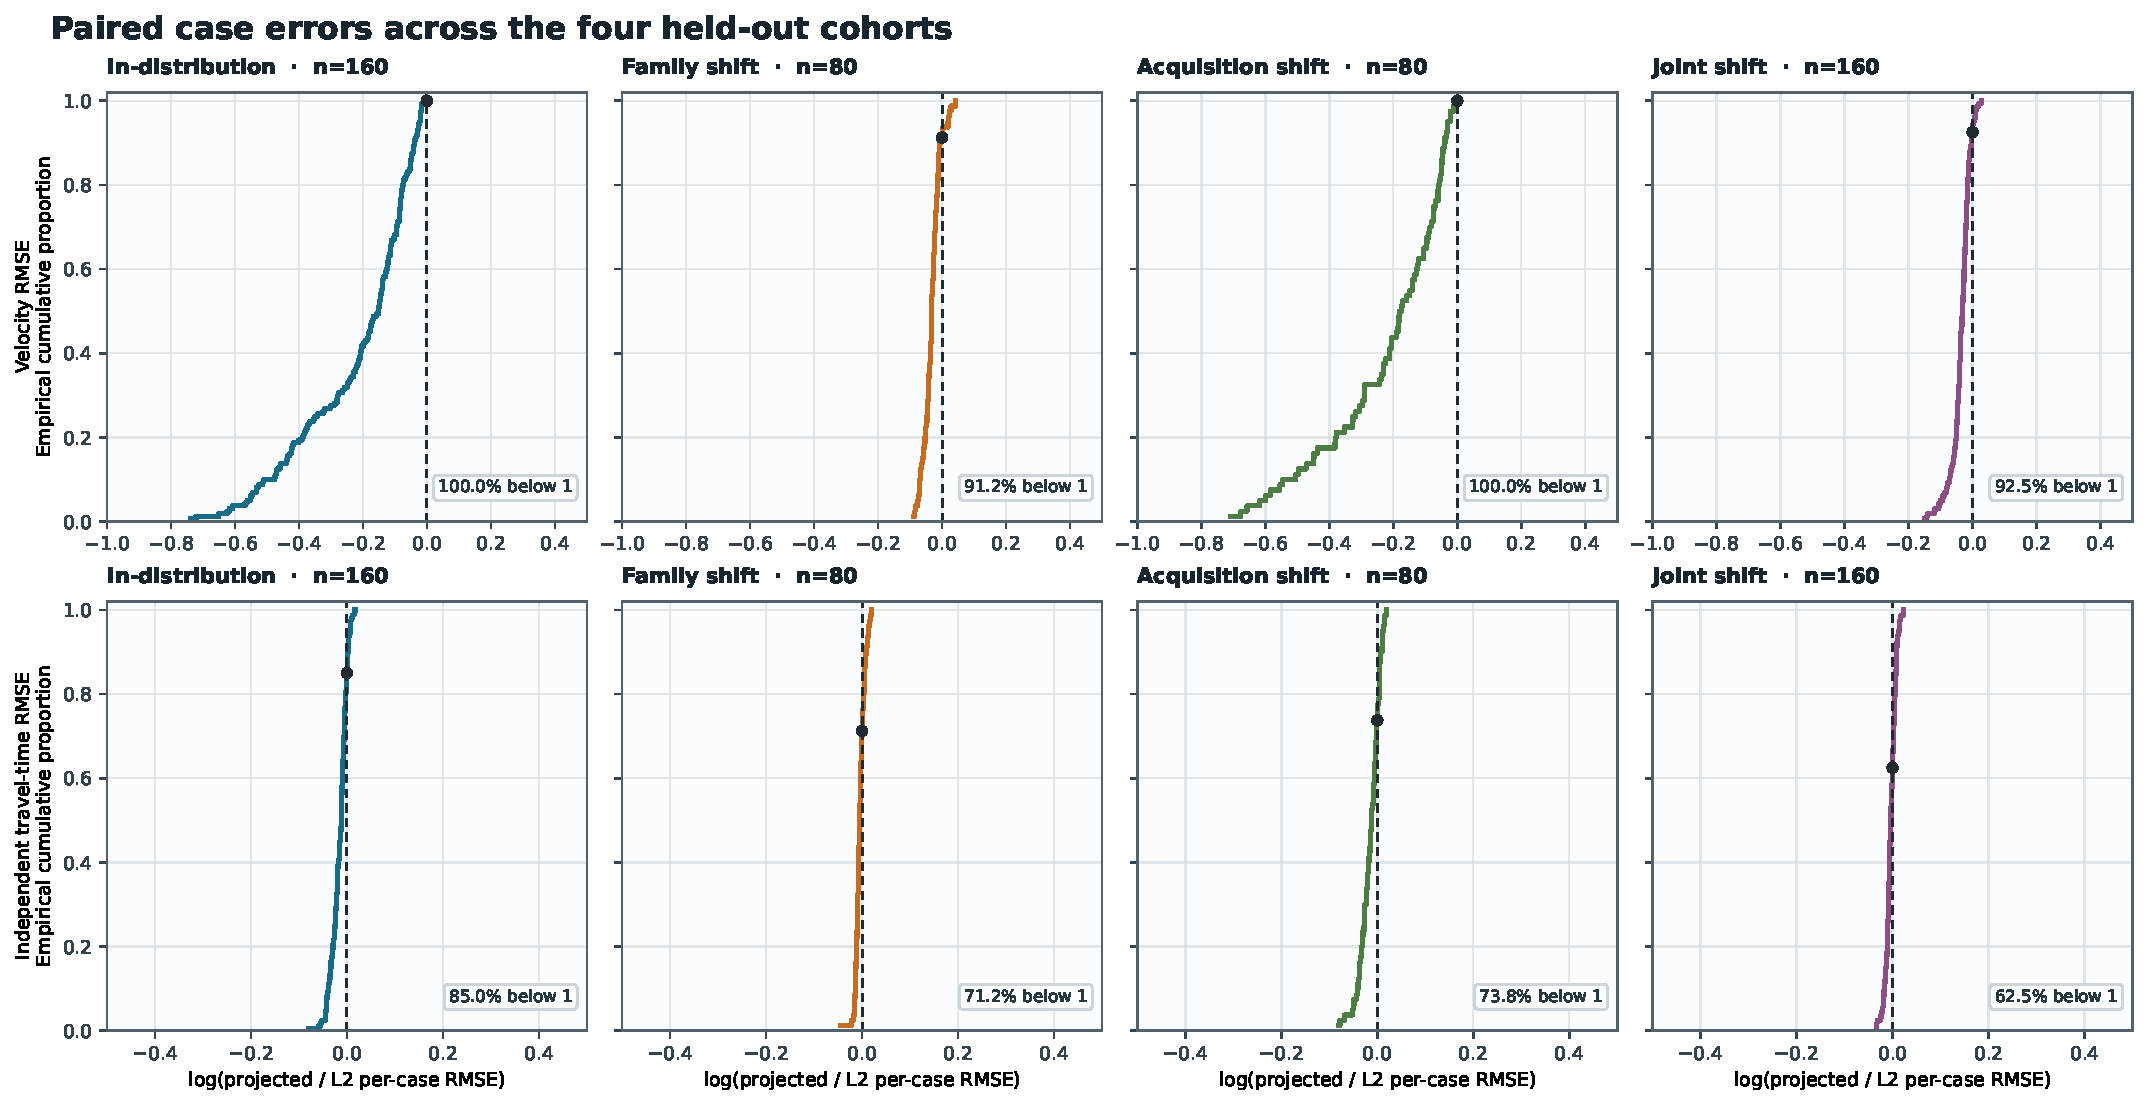
\includegraphics[width=\textwidth]{figures/m12-nullspace-paired-error-ecdf.pdf}
\caption{Empirical distributions of log paired per-case RMSE ratios across held-out cohorts, with zero marking equal projected and straight-ray L2 error.}
\label{fig:paired-ecdf}
\end{figure}

\begin{figure}[htbp]
\centering
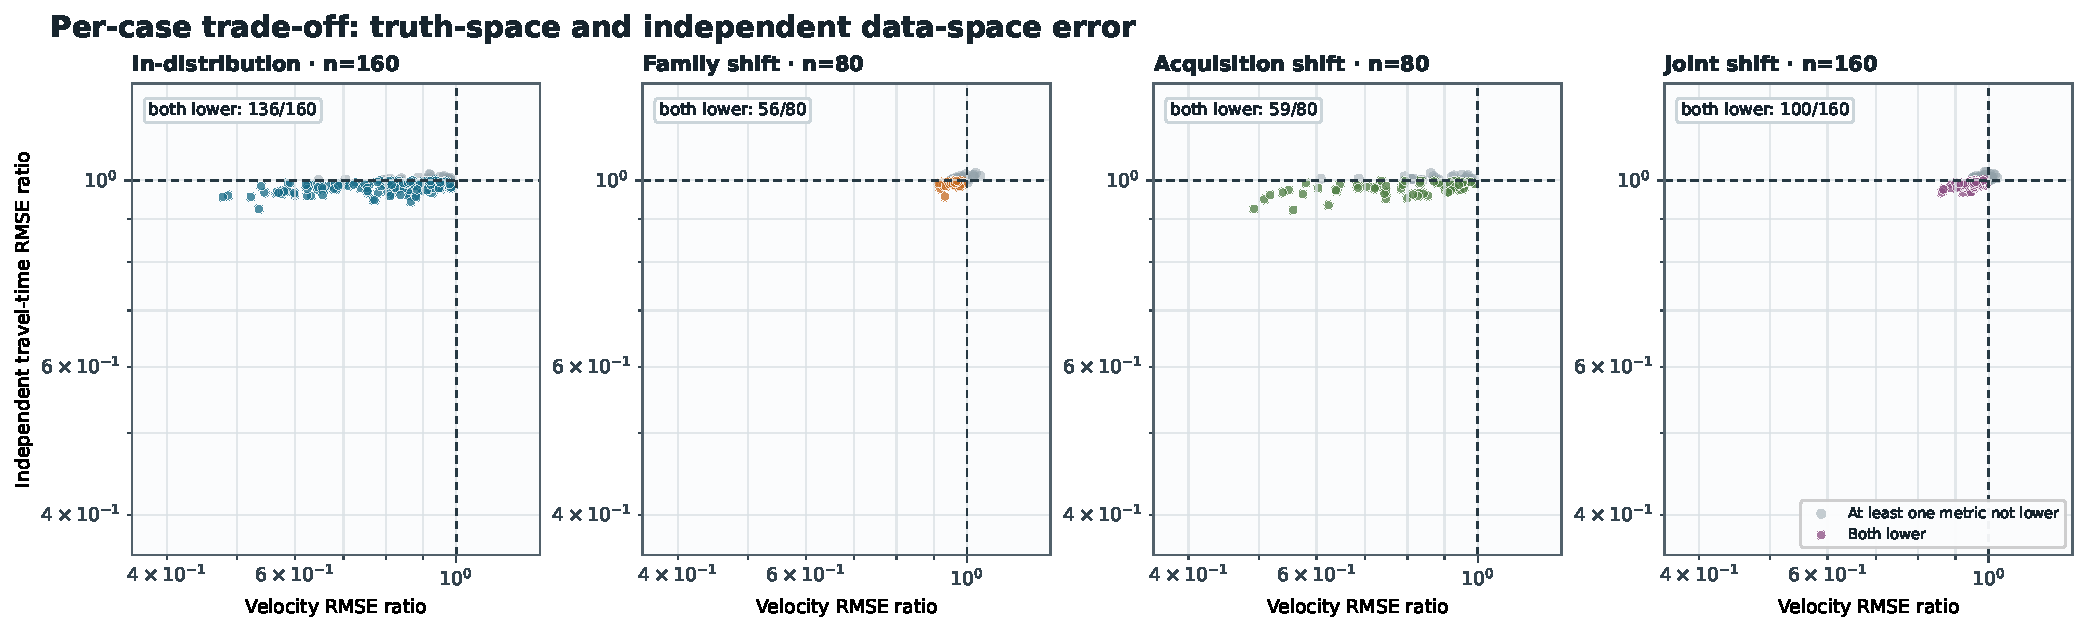
\includegraphics[width=\textwidth]{figures/m12-nullspace-case-error-tradeoffs.pdf}
\caption{Per-case velocity and independent travel-time RMSE ratios show whether each synthetic realization improves both criteria simultaneously.}
\label{fig:case-tradeoff}
\end{figure}

\begin{figure}[htbp]
\centering
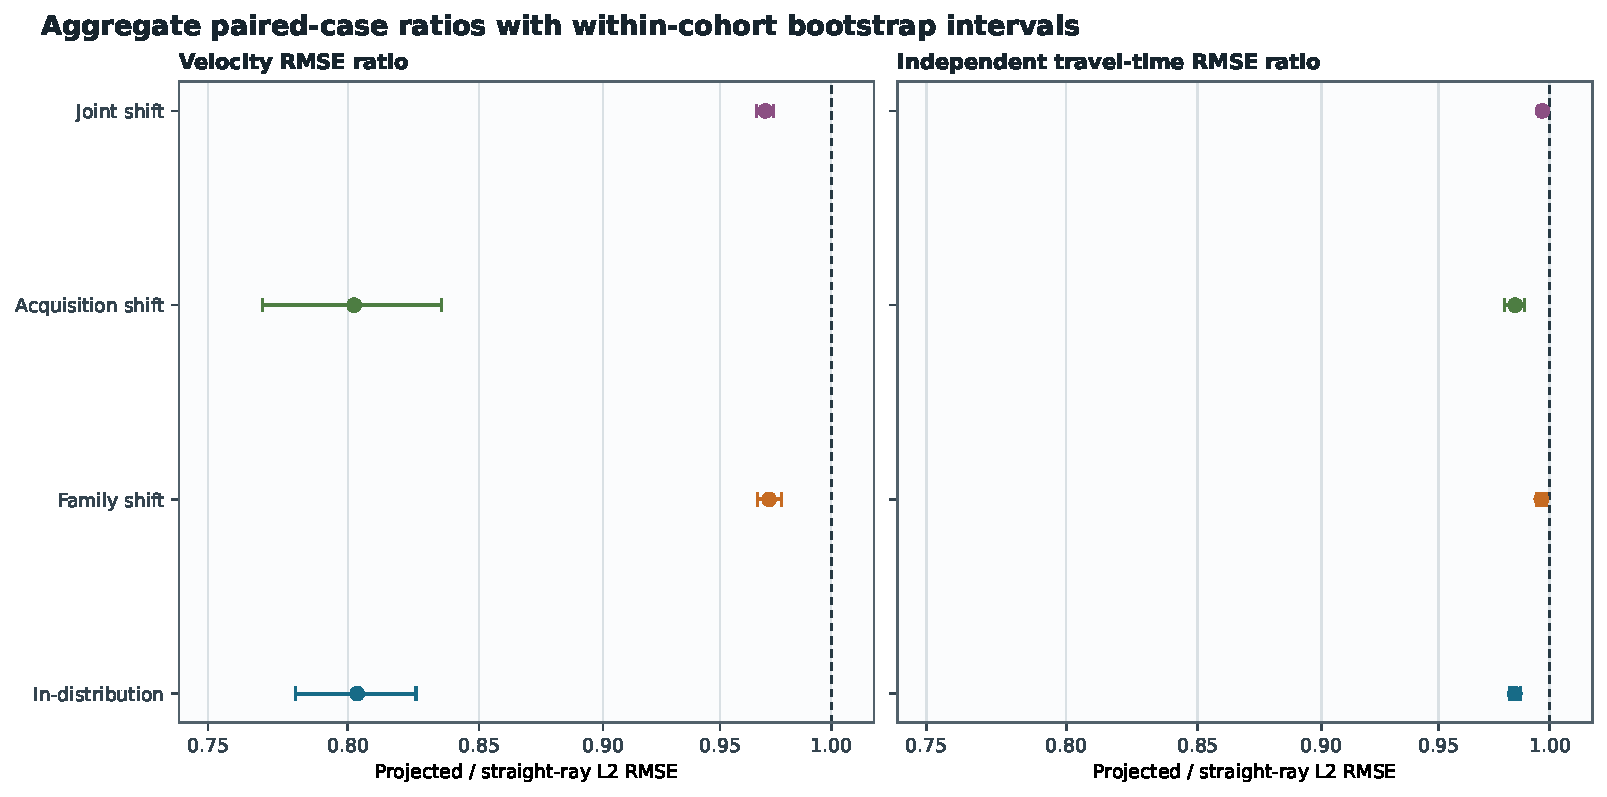
\includegraphics[width=0.98\textwidth]{figures/m12-nullspace-aggregate-ratio-intervals.pdf}
\caption{Aggregate paired-case RMSE ratios and percentile bootstrap intervals quantify variation within each fixed synthetic cohort.}
\label{fig:aggregate-intervals}
\end{figure}

\begin{figure}[htbp]
\centering
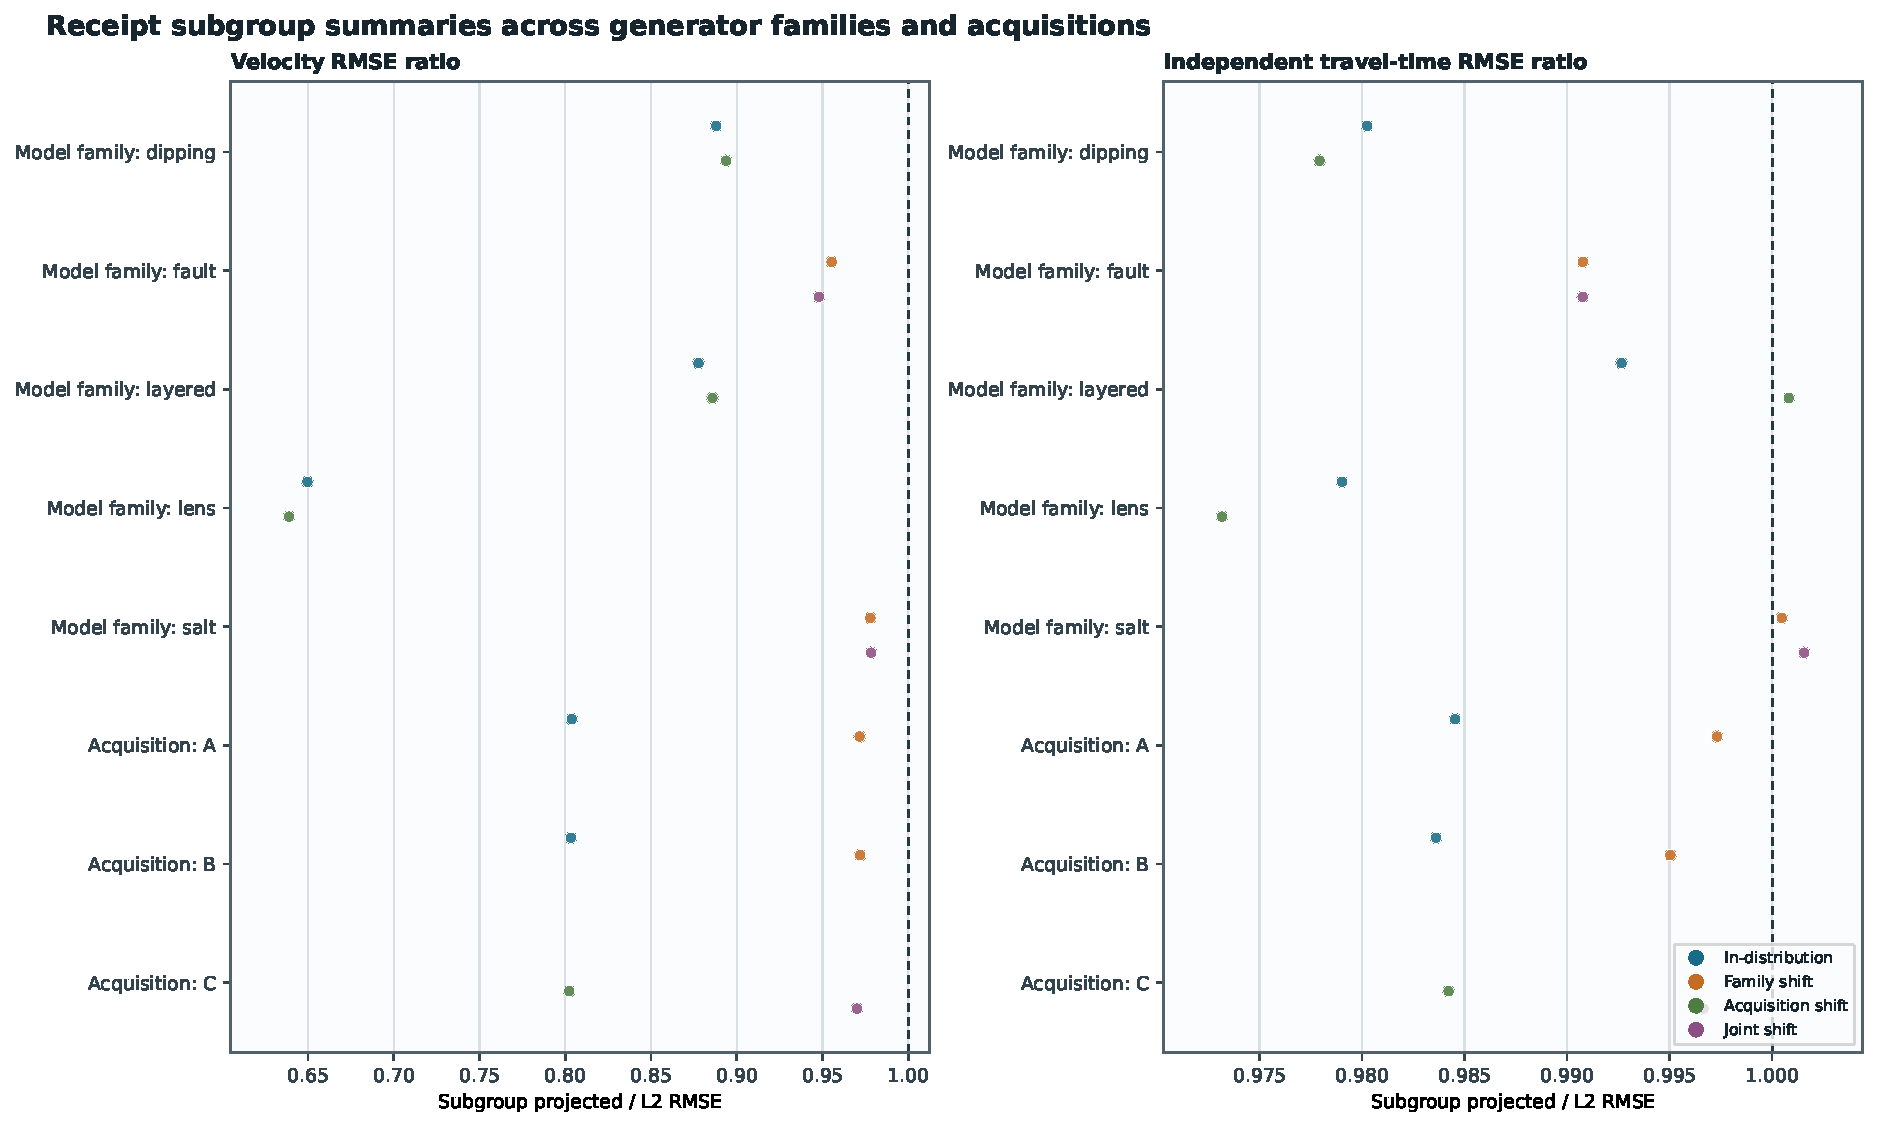
\includegraphics[width=\textwidth]{figures/m12-nullspace-subgroup-ratios.pdf}
\caption{Subgroup summaries separate generator-family and acquisition aggregates while retaining the shared cohort definitions in the held-out synthetic cohorts.}
\label{fig:subgroups}
\end{figure}

\begin{figure}[htbp]
\centering
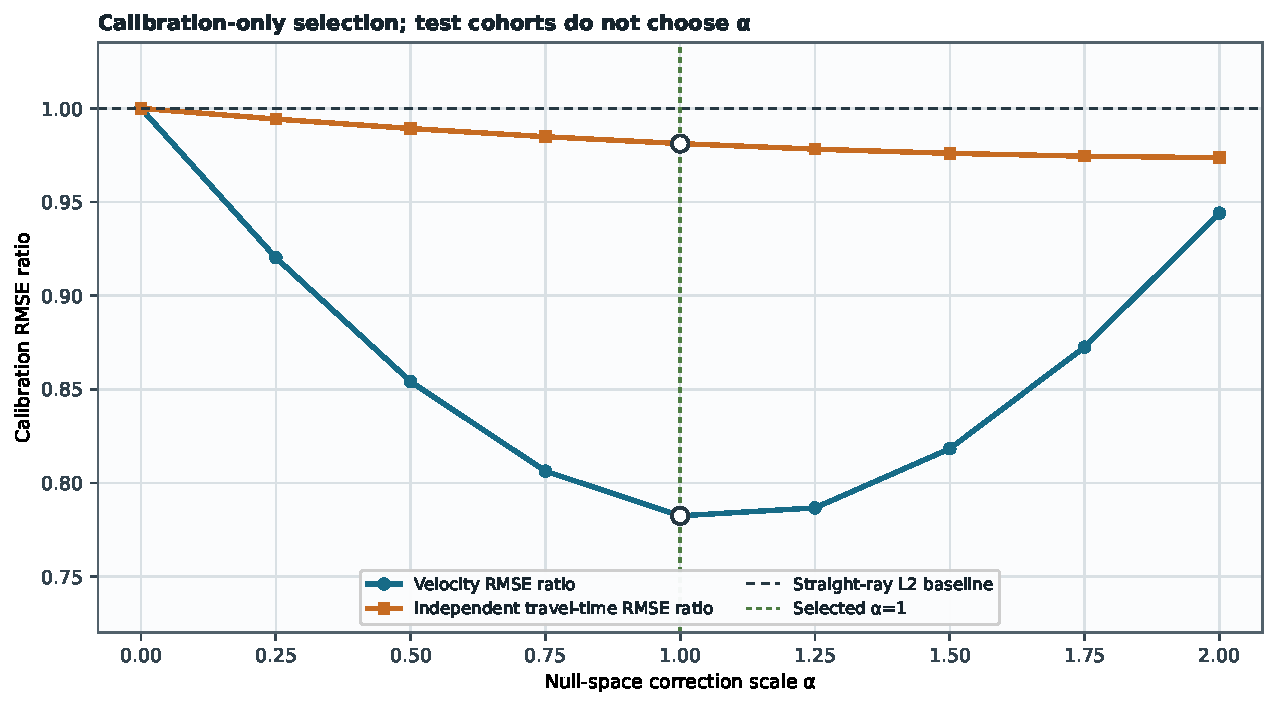
\includegraphics[width=0.9\textwidth]{figures/m12-nullspace-calibration-alpha-selection.pdf}
\caption{Calibration-only RMSE ratios over the correction grid identify the selected scale without using test-cohort outcomes.}
\label{fig:calibration}
\end{figure}

\begin{figure}[htbp]
\centering
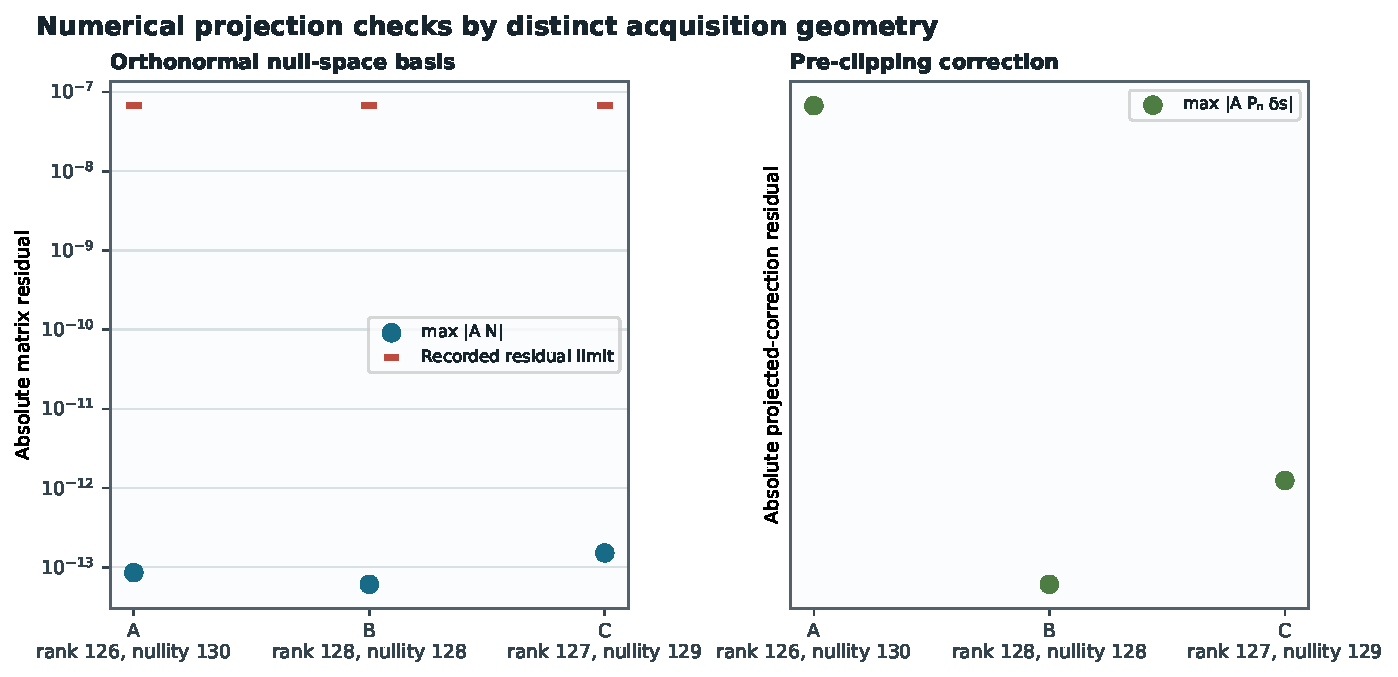
\includegraphics[width=0.9\textwidth]{figures/m12-nullspace-projection-diagnostics.pdf}
\caption{Recorded SVD basis and projected-correction residuals verify numerical null-space behavior for acquisition geometries A, B, and C in the synthetic experiment.}
\label{fig:projection-diagnostics}
\end{figure}

\subsection{Same-case projection ablation}
\label{sec:paired-ablation}
The projected-to-L2 ratios do not isolate the contribution of projection because the raw CNN was not one of their comparators. We regenerated raw and projected predictions from the same frozen checkpoint for each of the 480 follow-up test cases, holding the original calibration choices ($\alpha=1.0$, $\lambda=100$) fixed. The projected scores reproduce the v1.1 receipt. Table~\ref{tab:projection-counterfactual} and Figure~\ref{fig:projection-counterfactual} compare each case's velocity and independent-oracle errors; the bootstrap resamples case identifiers within each fixed cohort.

Projection lowers independent travel-time error relative to the raw CNN in all four cohorts. Its velocity effect is cohort-dependent: velocity error rises sharply in-distribution (ratio 1.9583) and under acquisition shift (1.8798), while falling under family shift (0.9143) and joint shift (0.9177). This is a metric trade-off for this checkpoint and simulator, not a uniform improvement. Because the analysis is post hoc and uses one checkpoint, one finite synthetic generator, and fixed discretizations, it does not establish performance over a geological population or a general benefit of null-space projection.

\begin{table}[htbp]
\centering
\scriptsize
\caption{Same-case projected-to-raw CNN error ratios and paired intervals quantify the correction trade-off across four frozen synthetic cohorts.}
\label{tab:projection-counterfactual}
\begin{tabular}{lrrrrr}
\toprule
Cohort & $n$ & Velocity ratio [95\% CI] & Lower & Oracle-time ratio [95\% CI] & Lower \\
\midrule
In distribution & 160 & 1.9583 [1.9070, 2.0113] & 0/160 & 0.9290 [0.9093, 0.9495] & 113/160 \\
Family shift & 80 & 0.9143 [0.9060, 0.9225] & 76/80 & 0.7013 [0.6830, 0.7207] & 80/80 \\
Acquisition shift & 80 & 1.8798 [1.8123, 1.9502] & 0/80 & 0.9146 [0.8900, 0.9400] & 57/80 \\
Joint shift & 160 & 0.9177 [0.9123, 0.9230] & 158/160 & 0.7080 [0.6954, 0.7213] & 160/160 \\
\bottomrule
\end{tabular}
\end{table}

\begin{figure}[htbp]
\centering
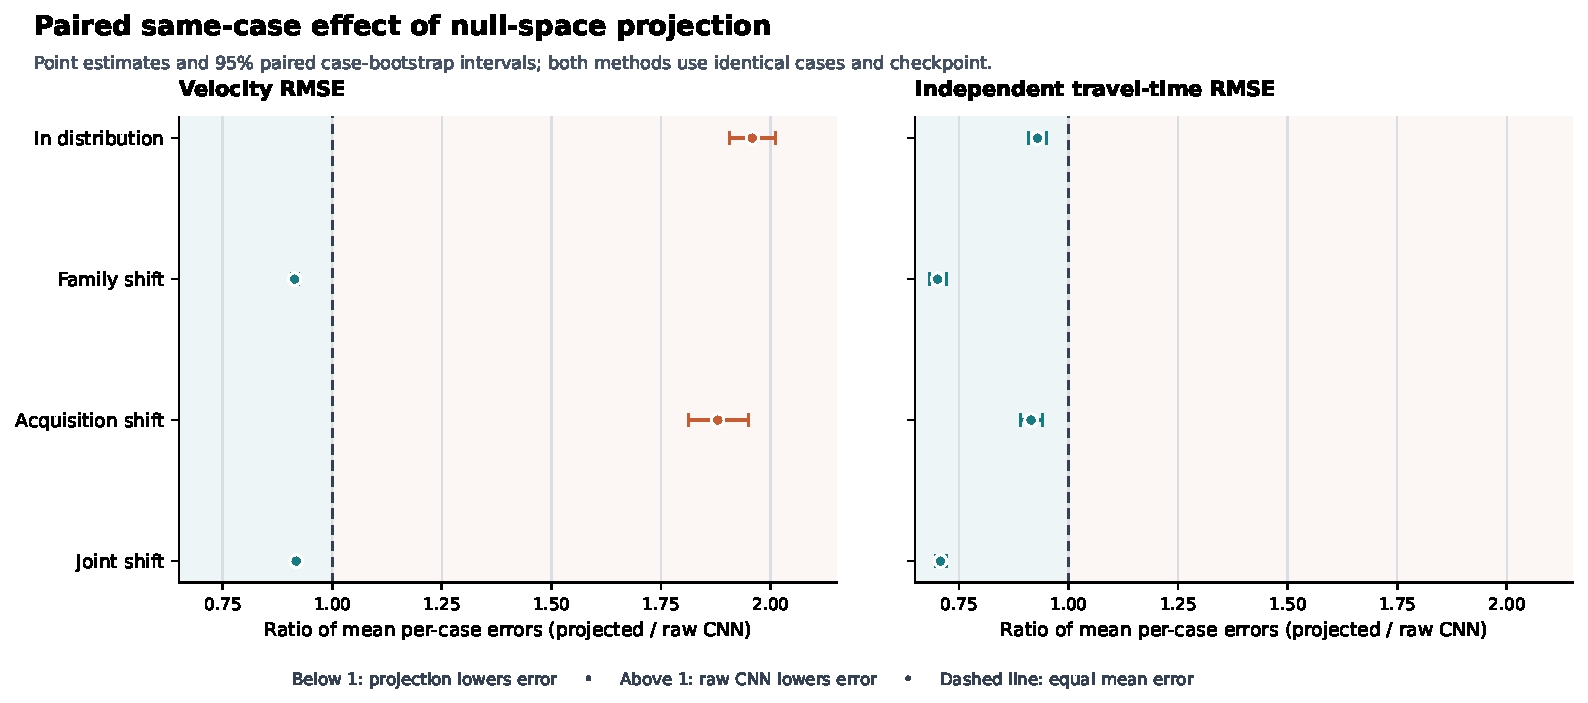
\includegraphics[width=0.98\textwidth]{figures/m12-projection-counterfactual.pdf}
\caption{Paired projected-to-raw CNN error ratios for the same cases in four frozen synthetic cohorts. The dashed line marks equal error; values below one favor projection for the named metric. Intervals resample cases within each cohort and are not population-level uncertainty.}
\label{fig:projection-counterfactual}
\end{figure}

\section{Relation to current methods and limits}
The literature contains at least three distinct learned tomography families relevant to comparison. Supervised inverse maps learn from model--data pairs and can exploit geometry-specific structure \cite{fan_ying_2023}. Physics-informed methods optimize velocity and travel-time fields against the eikonal equation and may include field applications \cite{waheed_2021, song_2025}. Neural parameterizations with ensemble Kalman inversion offer a different optimization and uncertainty strategy \cite{eki_nn_2024}. Null-space analysis itself has long-standing geophysical precedents \cite{pratt_1997,chave_2007}. A 2024 sparse-ray neural inversion study also reports a synthetic volcanic-edifice setting \cite{volcano_ann_2024}.

The study has two distinct comparisons. The original v1.1 receipt compares the projected candidate with the matched straight-ray L2 baseline; the post-hoc ablation compares projected and raw CNN predictions on the same follow-up cases. The latter isolates the computational intervention conditional on this frozen checkpoint, calibration and simulator, but it is not a prospective experiment and does not isolate effects across training seeds or generators. Neither comparison evaluates current published methods on common arrays, preprocessing, parameter tuning and scoring. This computation therefore does not reproduce or outperform the cited methods. A defensible external benchmark would require common data, implementations or faithful reproductions, matched information, and independent verification of every forward operator. The available evidence supports a bounded synthetic ablation, not a general causal or performance claim.

The positive ratios are conditional on synthetic families, a fixed grid, straight-ray projection, one inherited checkpoint, and the independent bilinear scoring operator. The base checkpoint already failed a separate locked comparison. The study has no field measurements, no external replication, no uncertainty calibration over geology, and no user-data benchmark. A small aggregate improvement does not imply sharper resolution, uniqueness, or correct structure. On the joint-shift cohort, the ratios correspond to about a 3.0\% velocity-RMSE decrease and a 0.33\% travel-time-RMSE decrease, whose practical significance is unknown. The difference between the two metrics is itself a limitation: velocity RMSE uses known synthetic truth, whereas travel-time RMSE evaluates agreement with a separate discretized operator. Neither is an estimate of field uncertainty or geological resolution.

The numerical projection check (Figure~\ref{fig:projection-diagnostics}) is a code-level consistency test for the chosen discretized path-length matrices. It says that the computed basis is close to the kernel of those matrices under the recorded tolerance and that the pre-clipping projected correction is numerically annihilated by the same operator. It does not assess whether the straight-ray matrix is a valid physical forward model for a heterogeneous medium, whether the test generator represents subsurface structure, or whether the learned correction contains useful geological information. The nonlinear velocity conversion and physical clipping occur after that linear check; independent travel-time evaluation is therefore essential and cannot be replaced by the $AN\approx0$ diagnostic. The per-geometry residuals in Table~\ref{tab:projection-diagnostics} are algebraic diagnostics, not observations of physical data-fit improvement.

\section{Discussion}\label{sec:discussion}
The same-case analysis changes the interpretation of the earlier projected-to-L2 table. That table shows that the projected candidate has lower cohort-average errors than the matched L2 estimate for both metrics in the four stored synthetic cohorts. It does not say whether the CNN contributed useful information, whether the projection corrected a flawed raw estimate, or whether projection itself caused the difference. The paired intervention answers the narrower conditional question: for these frozen weights, calibration and synthetic cases, how did applying the computed projector change the two errors? The results reveal that answer is not “better in every sense.” Travel-time error is lower after projection in every cohort, while velocity error increases in the ID and acquisition-only cohorts and decreases in the two cohorts that change geology family. The model and data metrics therefore express different consequences of the same transform.

The ID and acquisition-shift velocity increases are large, not a rounding artifact. Ratios near 1.9 mean the projected model's mean per-case velocity RMSE is roughly 90--96 percent larger than the raw CNN's in those cohorts. At the same time, the independent travel-time ratio below one indicates improved fit to the chosen oracle observations. This is compatible with movement toward a data-fitting direction that is less accurate with respect to the synthetic truth; data agreement and model recovery are distinct objectives in an underdetermined inverse problem. It is not evidence that the raw CNN is a better general inverse, because that model fails the separate frozen v3.1 joint-shift criterion. Nor is it evidence that the projected model's lower oracle error recovers the correct subsurface structure.

Under family shift and joint shift, projection lowers both metrics relative to raw CNN. This pattern may reflect interaction among the learned correction, the null-space basis and the generator's family distribution, but the current design does not identify a mechanism. The SVD basis is geometry-specific, and each acquisition layout produces a different row space. Family and layout factors are tested in four finite cohorts, with one training run and fixed held-out seeds. We cannot infer a robust treatment effect over unseen geologies, acquisition designs or network initializations. The bootstrap quantifies case-level variability conditional on those fixed factors only.

The result also highlights a practical control-design choice. Exact null-space projection prioritizes leaving the linearized $A$-predicted data unchanged in slowness space. A data-proximal method instead permits a bounded, explicitly chosen change to data fit; a trust-region or posterior method could trade model prior and data residual differently. Those alternatives are scientifically relevant follow-ups, but they would constitute new methods with new parameter selection and acceptance rules. They must not be inferred from this post-hoc ablation or introduced into the frozen v1.1 result. The present result is a diagnostic of one constrained post-processing operation, not a claim that exact null-space restriction is the optimal way to preserve evidence.

The synthetic scenario is also intentionally small relative to research benchmarks. It has four named test cohorts, one fixed grid, a limited family of authored shapes, fixed observation noise and known truth. This makes the case identities reproducible and permits independent scoring; it does not represent the structural, survey or processing diversity of field refraction work. Large FWI datasets such as OpenFWI show the value of multi-structure benchmark design for waveform inversion, but cannot replace task-matched first-arrival experiments. A future study should vary the number and diversity of families, noise distributions, topography, source and receiver layouts, ray bending and parameterization while locking test cohorts before training. It should compare at least a ray-updating or eikonal baseline and report common data-space, model-space and resolution diagnostics.

The manuscript therefore preserves two negative boundaries alongside the favorable projected-to-L2 result. First, residual-v3.1 remains a failed learned comparator on its original held-out test. Second, the v1.1 projected-to-L2 result, interpreted alongside its newly reproduced raw-CNN counterfactual, remains a bounded synthetic finding with scientific acceptance explicitly false. The incremental projection ratios are useful for understanding this record, but they do not reverse the v3.1 verdict, validate the simulator for field interpretation, or support a deployment claim.

\section{Limitations and validity threats}\label{sec:limitations}
The most important limitation is the absence of field observations and field acquisition metadata. Ground truth is available only because the cases are simulated. The noise model is controlled, the geology is authored, the model boundaries and reference trend are fixed, and the computational domain is rectangular. There are no real first-break picks, uncertain source coordinates, topography, anisotropy, attenuation, statics, correlated picking errors, out-of-plane rays, or survey-specific velocity bounds in this experiment. Thus, every error ratio is conditional on an artificial distribution and cannot be interpreted as field accuracy, usable resolution, or geological confidence.

The forward and inverse representations are deliberately different but both simplified. The straight-ray matrix $A$ is used to construct the L2 inverse and projection basis. The bilinear oracle is independently discretized and is used for the scored travel times. It is independent in implementation and discretization, not an independent physical validation dataset: both operators are applied to the same generated model and observations. The oracle also does not account for bent-ray propagation or full-wave effects. The difference between $A$ and $Q$ creates a controlled operator mismatch, which is useful for testing sensitivity to implementation choices but is not a complete uncertainty model for a real survey.

The comparison to L2 has finite scope. The selected quadratic regularization is not a universal optimum, and the study does not compare a broader suite of smoothness operators, sparsity penalties, Bayesian priors, refraction packages, eikonal solvers or full waveform methods on common data. Hyperparameters are selected from the declared calibration split, but that split does not cover every plausible geological or acquisition regime. The raw-to-projected comparison is post hoc: it was motivated by a missing counterfactual after the original outcome had been observed. Although the checkpoint, alpha, lambda, seeds and score calculation are fixed and no test-driven retuning occurs, this analysis should be treated as exploratory rather than as a preregistered confirmatory test.

There is one frozen learned checkpoint. Repeated predictions from that checkpoint on hundreds of cases do not replace independent training seeds. Architectural choices, optimization noise, training data resampling and checkpoint selection could materially alter raw and projected outputs. There is also no uncertainty ensemble or calibrated posterior. The paired case bootstrap addresses only sampling variation among cases within each fixed cohort. It does not propagate training uncertainty, model-selection uncertainty, operator error, generator uncertainty or field-domain shift. Future work needs repeated training runs nested within held-out geological families and acquisition layouts, with all model choices fixed before final evaluation.

The numerical null-space itself is conditional on the SVD cutoff, matrix scale and discretization. A finite-precision projector can leave a residual; rank can change under rescaling or near-threshold singular modes. The stored diagnostics confirm small residuals under the declared thresholds, but not robustness to alternative rank policies. Conversion from slowness to velocity is nonlinear; future applications with clipping or different physical bounds may change the final data error more strongly. The separate oracle catches one consequence for these tests, but does not prove invariance under other forward solvers.

Finally, the current conclusion is not a method-acceptance claim. The receipt retains \texttt{scientific\_acceptance=false}, and the app's broader method ladder, uploaded-data, host-capacity, owner, visual and release gates are separate. A scientifically interpretable local artifact does not by itself authorize a field survey, an online inverse service, or a public product release. Those stages need their own evidence and should not be inferred from this paper.

\section{Reproducibility and artifact scope}\label{sec:reproducibility}
The frozen source package contains the trained residual-v3.1 checkpoint, its training receipt, the null-space v1.1 receipt, the cohort seed manifests, the numerical source modules and the original per-case projected-to-L2 scores. Independent CPU verification regenerates five residual-study cohorts and four null-space cohorts from the retained source and seeds. The new paired analysis regenerates raw predictions for the exact four v1.1 test splits and recomputes projected predictions without changing the frozen alpha or lambda. It checks the projected score against the receipt before writing the paired result. This check guards against an accidentally different cohort, model or score function; it does not act as an independent implementation of the full method.

Each generated counterfactual record binds the checkpoint and source hashes, exact split manifests, runtime versions, bootstrap seed and per-case metrics. The figure and table are deterministic derivatives of this JSON receipt. Regeneration is performed outside the repository checkout to keep large transient arrays separate from source control; the compact JSON, plot, table source and file-hash manifest are retained with the manuscript. A reader can therefore distinguish the reproducible synthetic evidence from transient computation and from the separate CUDA training run.

Reproduction still has limits. The analysis depends on a specific Python environment and saved checkpoint; source hashing detects drift but does not prove that the code is correct. CPU replay confirms deterministic execution under this environment but does not validate independent numerical implementations, compiler portability or hardware equivalence beyond the tested CUDA-to-CPU chain. No claim is made that the generated notebook or app reruns this exact post-hoc analysis online. The public source repository provides code and artifacts; any result cited from this paper should retain the receipt and manifest identity rather than relying on the rendered figure alone.

\section{Conclusion}
On four fixed synthetic cohorts, the original projected-to-L2 comparison had lower aggregate velocity and independent travel-time RMSE. The paired ablation now shows that this does not mean projection uniformly improves the learned prediction: independent travel-time error falls in every cohort, while velocity error nearly doubles in-distribution and under acquisition shift and falls under family and joint shift. CUDA checkpoint regeneration, CPU verification, and the same-case analysis are reproducible from retained source, seeds and receipts. These results describe one frozen checkpoint, finite synthetic cohorts, and the declared discretized operators. They do not establish a new inverse algorithm, superiority over current methods, field accuracy, geological recovery, or generalization over a population. The earlier geometry-normalized CNN's locked joint-shift failure remains unchanged; the new analysis is an addition to the follow-up record, not a revised pass criterion. External claims require prospective multi-seed studies, independent method implementations, and field observations with documented physical corrections. A useful next experiment would preregister the geology families, acquisition layouts, noise and topographic perturbations, train multiple independent checkpoints, and compare raw, exactly projected and data-proximal corrections using a ray-updating solver alongside the independent oracle. Until such a study exists, the ratios should guide further experimental design only and must not be treated as expected performance for user-provided or field cases.

\section*{Data and code availability}
The implementation, synthetic cohort definitions, hash-identified data package, historical compatibility replay, bootstrap calculation, threshold reconciliation, figure generator and rendered figures are in the public source repository at \url{https://github.com/fsantibanezleal/CAOS_Geophysics}. The archived 2026-10-27 experiment-manifest SHA-256 is \texttt{30df0c2ad495bd850dda602b1c96725be8290dd086119fb3e8e75355fe9dea22}; generated figure hashes are listed in \texttt{figures/figure-manifest.json}. A 2026-11-06 current-source reproduction trained the residual-v3.1 checkpoint on CUDA and independently verified the residual and null-space runs on CPU. The checkpoint hash was \url{0f7a8fc43a078ab4cb16016774d44b356ccb70d9c60e0f197506fd3f7a53ea03}; the residual receipt hash was \url{f6f52c544af1a86f07fc17c83296de2ac09e884058e2af1d72adeb3bb35bc1dc}; and the null-space receipt hash was \url{0d4cd8c14e290b9cd17da387800dbe6cf7314729379d03221df8585b1243d880}. The outputs and a reproduction guide are retained under \url{data/derived/v2/models/m12-current-reproduction-20261106/}. Both verifiers returned \texttt{status=verified}; the residual model remains a failed held-out comparator and the null-space result remains supported only within its bounded synthetic protocol. The verifiers regenerate deterministic cohorts from the checked source and retained seeds. The 12 November post-hoc counterfactual regenerates raw and projected CNN predictions on identical cases, verifies projected-score parity with the v1.1 receipt, and stores per-case metrics and paired bootstrap intervals in \texttt{data/derived/v2/models/m12-projection-counterfactual-20261112/}. Its result is exploratory and does not change the original acceptance verdict. No field-data claim is made.

{\small
\begin{thebibliography}{99}
\bibitem{backus_gilbert_1968} G. Backus and F. Gilbert, ``The resolving power of gross Earth data,'' \emph{Geophysical Journal of the Royal Astronomical Society}, 16(2), 169--205, 1968. \href{https://doi.org/10.1111/j.1365-246X.1968.tb00216.x}{doi:10.1111/j.1365-246X.1968.tb00216.x}.
\bibitem{menke_2012} W. Menke, \emph{Geophysical Data Analysis: Discrete Inverse Theory}, 3rd ed., Academic Press, 2012.
\bibitem{aster_2018} R. C. Aster, B. Borchers, and C. H. Thurber, \emph{Parameter Estimation and Inverse Problems}, 3rd ed., Elsevier, 2018. \href{https://doi.org/10.1016/C2015-0-02458-3}{doi:10.1016/C2015-0-02458-3}.
\bibitem{vidale_1988} J. E. Vidale, ``Finite-difference calculation of travel times,'' \emph{Bulletin of the Seismological Society of America}, 78(6), 2062--2076, 1988.
\bibitem{hole_1992} J. A. Hole, ``Nonlinear high-resolution three-dimensional seismic travel time tomography,'' \emph{Journal of Geophysical Research: Solid Earth}, 97(B5), 6553--6562, 1992. \href{https://doi.org/10.1029/92JB00235}{doi:10.1029/92JB00235}.
\bibitem{podvin_lecomte_1991} P. Podvin and I. Lecomte, ``Finite difference computation of traveltimes in very contrasted velocity models: a massively parallel approach and its associated tools,'' \emph{Geophysical Journal International}, 105(1), 271--284, 1991. \href{https://doi.org/10.1111/j.1365-246X.1991.tb03461.x}{doi:10.1111/j.1365-246X.1991.tb03461.x}.
\bibitem{dahlen_2000} F. A. Dahlen, S.-H. Hung, and G. Nolet, ``Fr\'echet kernels for finite-frequency traveltimes---I. Theory,'' \emph{Geophysical Journal International}, 141(1), 157--174, 2000. \href{https://doi.org/10.1046/j.1365-246X.2000.00070.x}{doi:10.1046/j.1365-246X.2000.00070.x}.
\bibitem{dahlen_resolution_2004} F. A. Dahlen, ``Resolution limit of traveltime tomography,'' \emph{Geophysical Journal International}, 157(1), 315--331, 2004. \href{https://doi.org/10.1111/j.1365-246X.2004.02214.x}{doi:10.1111/j.1365-246X.2004.02214.x}.
\bibitem{pratt_1997} P. S. Rowbotham and R. G. Pratt, ``Improved inversion through use of the null space,'' \emph{Geophysics}, 62(3), 869--883, 1997. \href{https://doi.org/10.1190/1.1444195}{doi:10.1190/1.1444195}.
\bibitem{chave_2007} G. Mu\~noz and V. Rath, ``Beyond smooth inversion: the use of nullspace projection for the exploration of non-uniqueness in MT,'' \emph{Geophysical Journal International}, 164(2), 301--311, 2006. \href{https://doi.org/10.1111/j.1365-246X.2005.02825.x}{doi:10.1111/j.1365-246X.2005.02825.x}.
\bibitem{fan_ying_2023} Y. Fan and L. Ying, ``Solving traveltime tomography with deep learning,'' \emph{Communications in Mathematics and Statistics}, 11, 3--19, 2023. \href{https://doi.org/10.1007/s40304-022-00329-z}{doi:10.1007/s40304-022-00329-z}.
\bibitem{waheed_2021} U. B. Waheed, T. Alkhalifah, E. Haghighat, C. Song, and J. Virieux, ``PINNtomo: Seismic tomography using physics-informed neural networks,'' arXiv:2104.01588, 2021. \url{https://arxiv.org/abs/2104.01588}.
\bibitem{eki_nn_2024} Y. Li, Y. Zhang, X. Zhu, and J. Gao, ``Seismic traveltime tomography based on ensemble Kalman inversion,'' \emph{Geophysical Journal International}, 240(1), 290--302, 2025. \href{https://doi.org/10.1093/gji/ggae329}{doi:10.1093/gji/ggae329}.
\bibitem{volcano_ann_2024} A. Komeazi, G. R\"umpker, J. Faber, F. Limberger, and N. Srivastava, ``When linear inversion fails: Neural-network optimization for sparse-ray travel-time tomography of a volcanic edifice,'' \emph{Artificial Intelligence in Geosciences}, 5, 100086, 2024. \href{https://doi.org/10.1016/j.aiig.2024.100086}{doi:10.1016/j.aiig.2024.100086}.
\bibitem{song_2025} C. Song, H. Geng, Y. Wang, U. B. Waheed, and C. Liu, ``Simultaneous P- and S-wave seismic traveltime tomography using physics-informed neural networks,'' \emph{Geophysical Prospecting}, 73(6), e70034, 2025. \href{https://doi.org/10.1111/1365-2478.70034}{doi:10.1111/1365-2478.70034}.
\bibitem{msp_respinns_2026} Y. Xiang, Z. Song, Z. Wang, and G. Song, ``Residual Physics-Informed Neural Networks for Seismic Tomography with Multi-Source Prior Constraints,'' \emph{Mathematics}, 14(8), 1392, 2026. \href{https://doi.org/10.3390/math14081392}{doi:10.3390/math14081392}.
\bibitem{jacome_npn_2025} R. Jacome, R. Gualdr\'on-Hurtado, L. Su\'arez-Rodr\'iguez, and H. Arguello, ``NPN: Non-Linear Projections of the Null-Space for Imaging Inverse Problems,'' in \emph{Advances in Neural Information Processing Systems 38}, 2025. \href{https://doi.org/10.52202/085713-3973}{doi:10.52202/085713-3973}.
\bibitem{bacca_projection_2025} J. Bacca, ``Projection-Based Correction for Enhancing Deep Inverse Networks,'' arXiv:2505.15777, 2025. \url{https://arxiv.org/abs/2505.15777}.
\bibitem{aki_lee_1976} K. Aki and W. H. K. Lee, ``Determination of three-dimensional velocity anomalies under a seismic array using first P arrival times from local earthquakes: 1. A homogeneous initial model,'' \emph{Journal of Geophysical Research}, 81(23), 4381--4399, 1976. \href{https://doi.org/10.1029/JB081i023p04381}{doi:10.1029/JB081i023p04381}.
\bibitem{rawlinson_sambridge_2003} N. Rawlinson and M. Sambridge, ``Seismic traveltime tomography of the crust and lithosphere,'' \emph{Advances in Geophysics}, 46, 81--198, 2003. \href{https://doi.org/10.1016/S0065-2687(03)46002-0}{doi:10.1016/S0065-2687(03)46002-0}.
\bibitem{zelt_barton_1998} C. A. Zelt and P. J. Barton, ``Three-dimensional seismic refraction tomography: A comparison of two methods applied to data from the Faeroe Basin,'' \emph{Journal of Geophysical Research: Solid Earth}, 103(B4), 7187--7210, 1998. \href{https://doi.org/10.1029/97JB03536}{doi:10.1029/97JB03536}.
\bibitem{zelt_resolution_1998} C. A. Zelt, ``Lateral velocity resolution from three-dimensional seismic refraction data,'' \emph{Geophysical Journal International}, 135(3), 1101--1112, 1998. \href{https://doi.org/10.1046/j.1365-246X.1998.00695.x}{doi:10.1046/j.1365-246X.1998.00695.x}.
\bibitem{pinneik_2021} U. B. Waheed, E. Haghighat, T. Alkhalifah, C. Song, and Q. Hao, ``PINNeik: Eikonal solution using physics-informed neural networks,'' \emph{Computers \& Geosciences}, 155, 104833, 2021. \href{https://doi.org/10.1016/j.cageo.2021.104833}{doi:10.1016/j.cageo.2021.104833}.
\bibitem{openfwi_2022} C. Deng, S. Feng, H. Wang, X. Zhang, P. Jin, Y. Feng, Q. Zeng, Y. Chen, and Y. Lin, ``OpenFWI: Large-scale multi-structural benchmark datasets for full waveform inversion,'' in \emph{Advances in Neural Information Processing Systems 35, Datasets and Benchmarks Track}, 2022. \href{https://doi.org/10.52202/068431-0435}{doi:10.52202/068431-0435}.
\bibitem{goeppel_2023} S. G\"oppel, J. Frikel, and M. Haltmeier, ``Data-proximal null-space networks for inverse problems,'' arXiv:2309.06573, 2023. \url{https://arxiv.org/abs/2309.06573}.
\end{thebibliography}
}
\end{document}
